\section{Banco de Animales}
En un universo de fábula, los animales llevan la cuenta de su dinero en el banco internacional de animales. La familia Pythoninae (formada por pitones), dueña del banco, lleva el registro de la selva en un programa con lenguaje Python, pero al no tener dedos para programar, decide encargarle esta tarea a los humanos que estudian IWI-131 en el CIAC. Para ello se tienen las siguientes estructuras:

\begin{lstlisting}[style=consola]
animales=[
    #(nombre cientifico, nombre comun, f_nacimiento,correo)
    ('Panthera tigris','tigre',(1972,7,20),'tiger@animail.in'),
    ('Vultur gryphus','condor',(1989,4,27),'condorito@pelotillehue.cl'),
    ('Macropus fuliginosus','canguro',(1986,10,18),'rocko@animail.au'),
    ('Elephas maximus','elefante asiatico',(1973,11,10),'lfant@chinchan.wan.cn'),
    ('Loxodonta africana','elefante africano',(1993,7,8),'orejon@wakawaka.za')
    ]

paises={
    'in':'India',
    'cl':'Chile',
    'au':'Australia',
    'cn':'China',
    'za':'Sudafrica',
    'ar':'Argentina',
    'ch':'Suiza'
    }
    
meses=['enero','febrero','marzo','abril','mayo','junio','julio',
       'agosto','septiembre','octubre','noviembre','diciembre']

\end{lstlisting}

Y un archivo de texto
\begin{figure}[h]
    \centering
    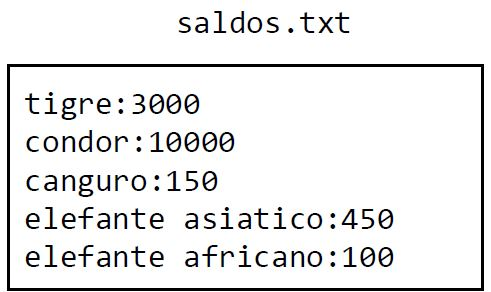
\includegraphics[scale=0.6]{Imagenes/imagen4.jpg}
\end{figure}

Se le pide a usted programar las siguientes funciones:

\begin{itemize}
    \item[a.] \texttt{listaPaises(animales)} que reciba la lista de animales y retorna una lista con todos los paises que usan el banco. Para esto debe usar el TLD, que es la parte de la dirección del correo electrónico que está después del último punto.
    \begin{lstlisting}[style=consola]
>>> listaPaises(animales)
['India','Chile','Australia','China','Sudafrica']    
    \end{lstlisting}
    \item[b.] \texttt{animalMasJoven(animales)} que reciba la lista de animales y retorne un string con el nombre científico del animal más joven.
    \begin{lstlisting}[style=consola]
>>> animalMasJoven(animales)
'Loxodonta africana'
    \end{lstlisting}
    \item[c.] \texttt{obtenerCumpleaneros(animales,mes)} que reciba la lista de animales y un string con el mes a buscar y retorne un conjunto con los correos electrónicos de los animales que estén de cumpleaños para \textst{llenarlos de SPAM} felicitarlos oportunamente. Nótese que el mes se expresa con palabras y no con números.
    \begin{lstlisting}[style=consola]
>>> obtenerCumpleaneros(animales,'julio')
set(['orejon@wakawaka.za', 'tiger@animail.in'])
    \end{lstlisting}
    \item[d.] \texttt{depositar(animal,monto,archivo)} que reciba el nombre común de un animal, un entero con el monto a depositar y el nombre del archivo con los saldos para modificar el archivo con el nuevo saldo del animal. Asuma que hay muchos animales en el mundo, tal que es imposible guardar sus datos en una estructura de tipo lista, conjunto, diccionario o tupla.
    \begin{lstlisting}[style=consola]
>>> depositar('canguro',10,'saldos.txt')
Deposito realizado con exito!
    \end{lstlisting}
    \item[e.] \texttt{sacarDinero(animal,monto,archivo)} que reciba el nombre común de un animal, un entero con el monto a girar y el nombre del archivo con los saldos para modificar el archivo con el nuevo saldo del animal. Siga asumiendo que su computador explotará si usa listas, tuplas, conjuntos o diccionarios.
    \begin{lstlisting}[style=consola]
>>>sacarDinero('canguro',200,'saldos.txt')
No se puede realizar giro

>>>sacarDinero('condor',100,'saldos.txt')
Giro realizado con exito!
    \end{lstlisting}
\end{itemize}